\PassOptionsToPackage{unicode=true}{hyperref} % options for packages loaded elsewhere
\PassOptionsToPackage{hyphens}{url}
%
\documentclass[10pt,ignorenonframetext,]{beamer}
\usepackage{pgfpages}
\setbeamertemplate{caption}[numbered]
\setbeamertemplate{caption label separator}{: }
\setbeamercolor{caption name}{fg=normal text.fg}
\beamertemplatenavigationsymbolsempty
\usepackage{lmodern}
\usepackage{amssymb,amsmath}
\usepackage{ifxetex,ifluatex}
\usepackage{fixltx2e} % provides \textsubscript
\ifnum 0\ifxetex 1\fi\ifluatex 1\fi=0 % if pdftex
  \usepackage[T1]{fontenc}
  \usepackage[utf8]{inputenc}
  \usepackage{textcomp} % provides euro and other symbols
\else % if luatex or xelatex
  \usepackage{unicode-math}
  \defaultfontfeatures{Ligatures=TeX,Scale=MatchLowercase}
\fi
\usetheme[]{Malmoe}
% use upquote if available, for straight quotes in verbatim environments
\IfFileExists{upquote.sty}{\usepackage{upquote}}{}
% use microtype if available
\IfFileExists{microtype.sty}{%
\usepackage[]{microtype}
\UseMicrotypeSet[protrusion]{basicmath} % disable protrusion for tt fonts
}{}
\IfFileExists{parskip.sty}{%
\usepackage{parskip}
}{% else
\setlength{\parindent}{0pt}
\setlength{\parskip}{6pt plus 2pt minus 1pt}
}
\usepackage{hyperref}
\hypersetup{
            pdftitle={Estimating the Effect of Discretion in Public Spending on Government Performance:},
            pdfauthor={Andre Assumpcao; Ciro Biderman; George Avelino},
            pdfborder={0 0 0},
            breaklinks=true}
\urlstyle{same}  % don't use monospace font for urls
\newif\ifbibliography
\usepackage{graphicx,grffile}
\makeatletter
\def\maxwidth{\ifdim\Gin@nat@width>\linewidth\linewidth\else\Gin@nat@width\fi}
\def\maxheight{\ifdim\Gin@nat@height>\textheight\textheight\else\Gin@nat@height\fi}
\makeatother
% Scale images if necessary, so that they will not overflow the page
% margins by default, and it is still possible to overwrite the defaults
% using explicit options in \includegraphics[width, height, ...]{}
\setkeys{Gin}{width=\maxwidth,height=\maxheight,keepaspectratio}
% Prevent slide breaks in the middle of a paragraph:
\widowpenalties 1 10000
\raggedbottom
\setbeamertemplate{part page}{
\centering
\begin{beamercolorbox}[sep=16pt,center]{part title}
  \usebeamerfont{part title}\insertpart\par
\end{beamercolorbox}
}
\setbeamertemplate{section page}{
\centering
\begin{beamercolorbox}[sep=12pt,center]{part title}
  \usebeamerfont{section title}\insertsection\par
\end{beamercolorbox}
}
\setbeamertemplate{subsection page}{
\centering
\begin{beamercolorbox}[sep=8pt,center]{part title}
  \usebeamerfont{subsection title}\insertsubsection\par
\end{beamercolorbox}
}
\AtBeginPart{
  \frame{\partpage}
}
\AtBeginSection{
  \ifbibliography
  \else
    \frame{\sectionpage}
  \fi
}
\AtBeginSubsection{
  \frame{\subsectionpage}
}
\setlength{\emergencystretch}{3em}  % prevent overfull lines
\providecommand{\tightlist}{%
  \setlength{\itemsep}{0pt}\setlength{\parskip}{0pt}}
\setcounter{secnumdepth}{0}

% set default figure placement to htbp
\makeatletter
\def\fps@figure{htbp}
\makeatother


\title{Estimating the Effect of Discretion in Public Spending on Government
Performance:}
\providecommand{\subtitle}[1]{}
\subtitle{Evidence from Brazilian Municipalities}
\author{Andre Assumpcao \and Ciro Biderman \and George Avelino}
\providecommand{\institute}[1]{}
\institute{UNC Chapel Hill, FGV-EAESP, FGV-EAESP}
\date{Oct 13th, 2018}

\begin{document}
\frame{\titlepage}

\begin{frame}{Motivation}
\protect\hypertarget{motivation}{}

Developing countries spend \textbf{US\$820bn} per year on goods and
services supplied by the private sector. Governments purchase medical
supplies, school material, and construction services used to implement
public policies.

Constituents thus have an interest not only on \textbf{what} goods and
services governments are purchasing but also \textbf{how} governments
are acquiring such items.

\begin{itemize}
\item
  When will the town build better access roads?
\item
  Should the government ask for three budget proposals for a school
  project or just one?
\item
  How many insulin injections should be purchased given their expiry
  date and the number of people who need them?
\end{itemize}

\end{frame}

\begin{frame}{Research Question}
\protect\hypertarget{research-question}{}

\emph{Does the imposition of harder, stricter procurement rules for
government expenditure reduce corruption and misallocation of public
resources?}

\textbf{Context}

Random sample of 9,593 federal transfers to 1,139 Brazilian
municipalities, between 2004-2010, to cover health and education
expenditures for which we construct or collect data on:

\begin{itemize}
\item
  Corruption and mismanagement (\textbf{outcomes})
\item
  Procurement discretion (\textbf{treatments})
\item
  Municipal characteristics (\textbf{controls})
\end{itemize}

\end{frame}

\begin{frame}{Hypotheses}
\protect\hypertarget{hypotheses}{}

\begin{enumerate}
\item
  The imposition of harder, stricter procurement rules for public
  spending \textbf{reduces} corruption.
\item
  The imposition of harder, stricter procurement rules for public
  spending \textbf{reduces} the misallocation of public resources.
\end{enumerate}

\textbf{Findings}

\begin{enumerate}
\item
  Stricter procurement rules have \textbf{no effect} on corruption.
\item
  Stricter procurement rules have only a \textbf{limited effect} on
  mismanagement.
\end{enumerate}

\end{frame}

\begin{frame}{Empirical Strategy}
\protect\hypertarget{empirical-strategy}{}

\textbf{Regression discontinuity (RD)} where the application of
procurement rules follows a strict monetary schedule established by Law
8,666/93.

\begin{figure}
\centering
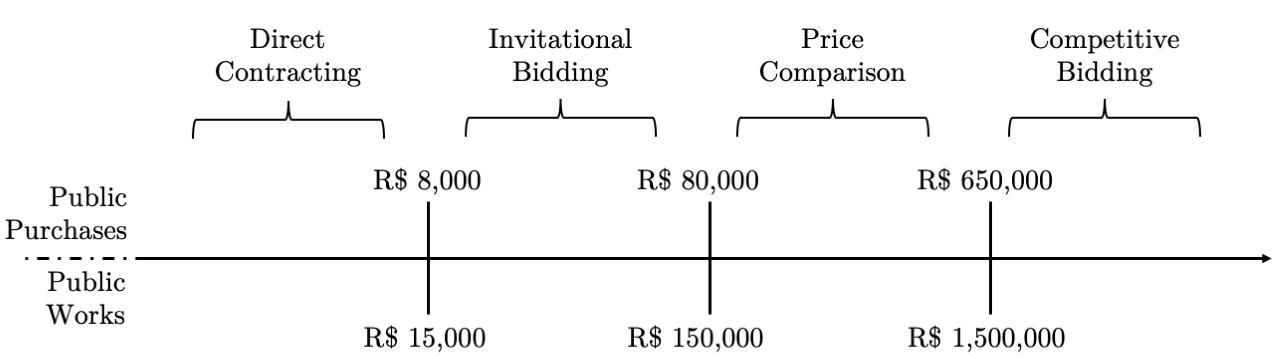
\includegraphics{./images/procurement_schedule.png}
\caption{Law 8,666/93}
\end{figure}

Looking at federal transfers whose values fall in the vicinities of the
discontinuities in procurement rules allows for the identification of
the \textbf{causal effect} of discretion on government performance.

\end{frame}

\begin{frame}{Outcomes}
\protect\hypertarget{outcomes}{}

The Office of the Comptroller-General (CGU) ran a random audit program
of Brazilian municipalities expenditures between 2003 and 2015, which we
use to code corruption and misallocation indicators serving as outcome
variables in this project (Ferraz and Finan, 2008; 2011).

\begin{itemize}
\item
  \textbf{Binary:} whether the transfer contains evidence of corruption
  or mismanagement;
\item
  \textbf{Share:} how many of each transfer's records are corruption or
  mismanagement-related;
\item
  \textbf{Amount:} how much money was potentially lost to corruption or
  mismanagement.
\end{itemize}

In total, my preferred estimation yields 6 (outcomes) \emph{x} {[}2
(purchases cutoffs) + 3 (works cutoffs) + 3 (pooled cutoffs){]} = 48
parameter estimates.

\end{frame}

\begin{frame}{Results}
\protect\hypertarget{results}{}

\begin{figure}
\centering
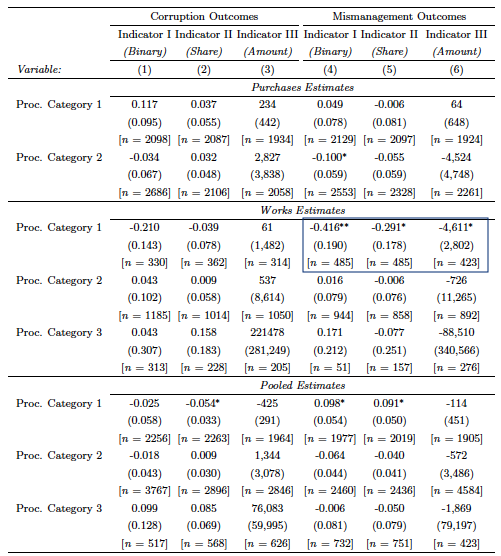
\includegraphics[width=0.7\textwidth,height=\textheight]{./images/table.png}
\caption{RD parameter estimates}
\end{figure}

\end{frame}

\begin{frame}{Mismanagement Binary}
\protect\hypertarget{mismanagement-binary}{}

\begin{figure}
\centering
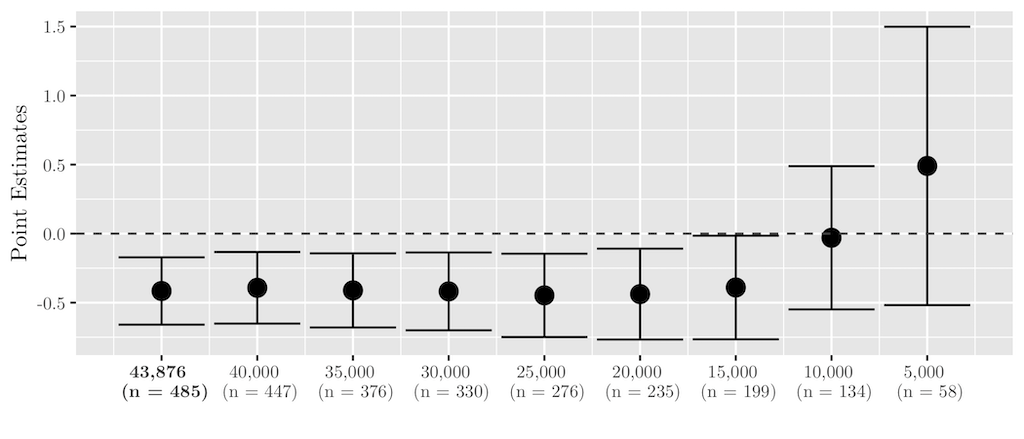
\includegraphics{./images/mismanagementplot1.png}
\caption{Outcome 1}
\end{figure}

\textbf{Interpretation:} reducing the discretion with which public
agents hire private contractors for public works projects reduces the
probability that these will be subject to mismanagement by \textbf{41.9
percentage points}.

\end{frame}

\begin{frame}{Results are robust!}
\protect\hypertarget{results-are-robust}{}

\begin{enumerate}
\item
  We run covariate balance tests across cutoffs and include covariates
  in regressions.
\item
  We use robust standard errors, clustered at the municipal level, and
  health, education, and auditing fixed effects.
\item
  We run the McCrary (2008) test for manipulation of the running
  variable and throw away the last cutoff in the goods/services
  procurement type.
\item
  Optimal bandwidth selection comes from Calonico, Cattaneo, and
  Titiunik (2015), but we also run our local (quadratic) regressions at
  smaller bandwidths.
\item
  There are two falsification tests showing that our significant
  mismanagement effects are not spurious\ldots{}
\end{enumerate}

\end{frame}

\begin{frame}{Falsification Tests 1}
\protect\hypertarget{falsification-tests-1}{}

Is this result spurious? Using \textbf{fake purchases} cutoffs for works
transfers, the answer is \textbf{no}.

\begin{figure}
\centering
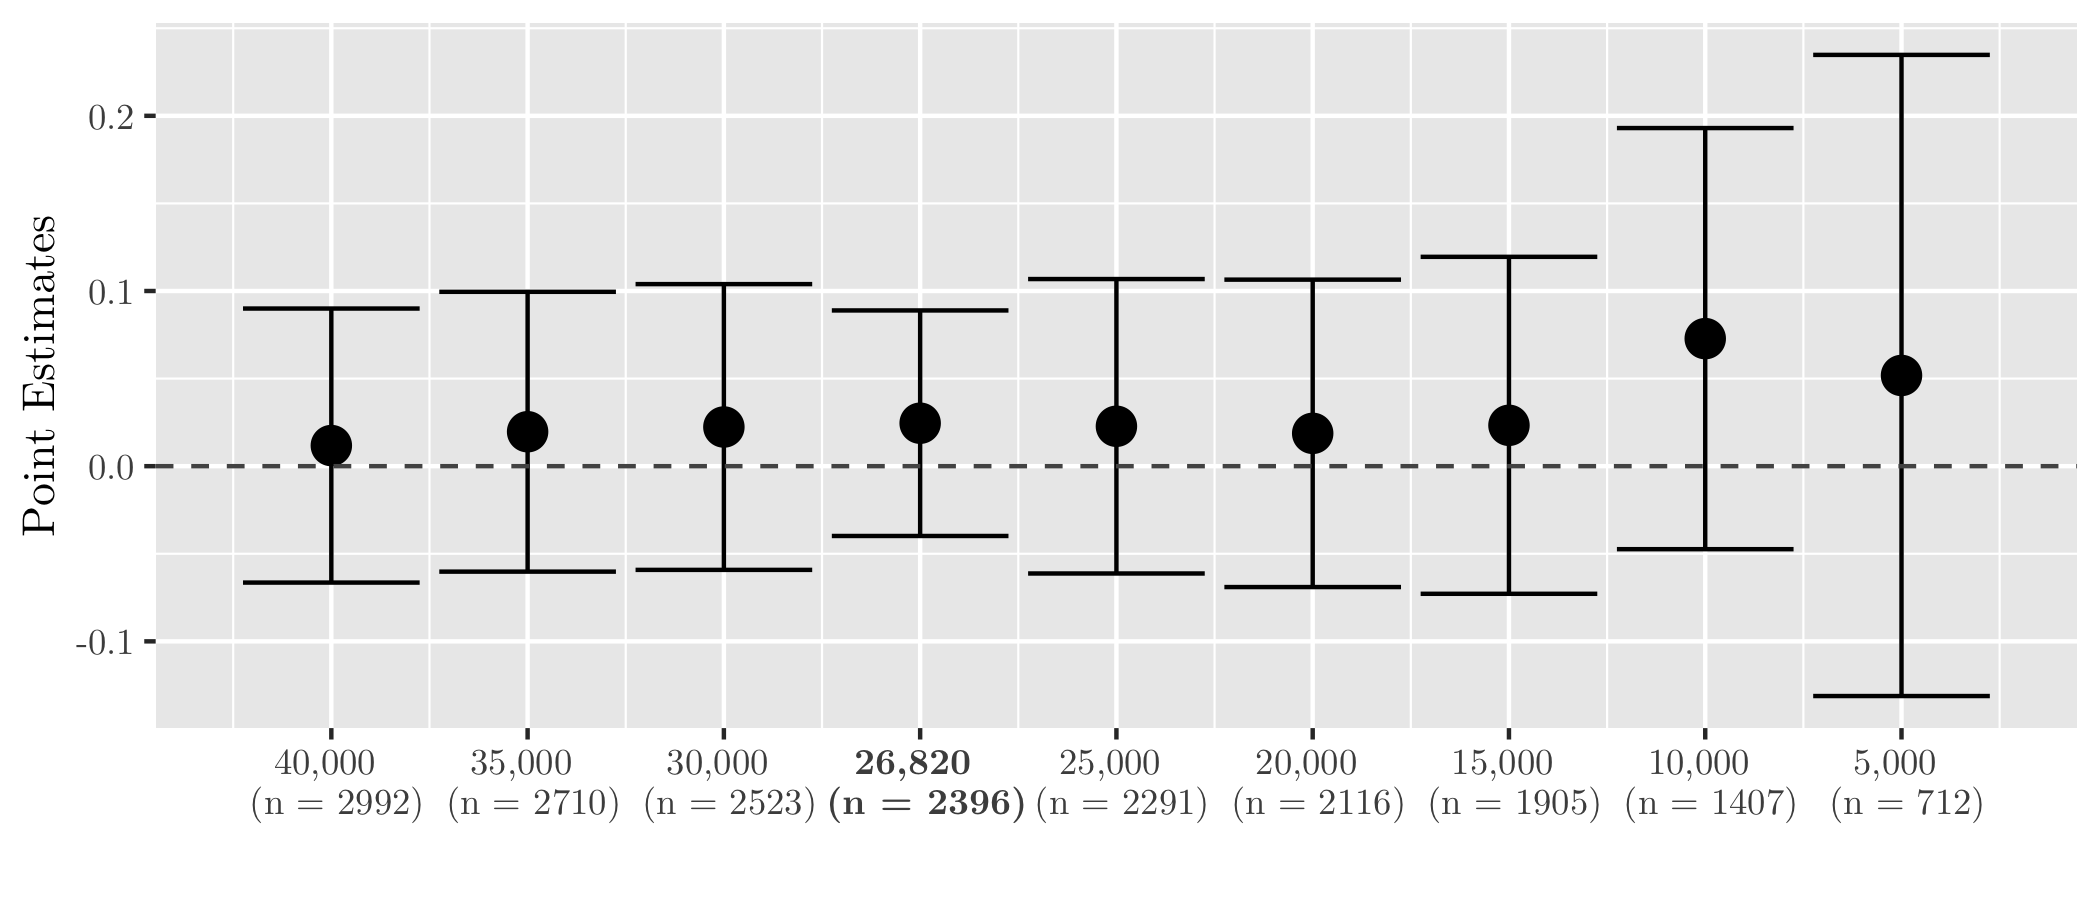
\includegraphics{./images/01falsificationplot1.png}
\caption{Mismanagement Binary Placebo 1}
\end{figure}

\end{frame}

\begin{frame}{Falsification Tests 2}
\protect\hypertarget{falsification-tests-2}{}

Isn't this just a random discontinuity due to chance? Using
\textbf{non-procurement} transfers, the answer is also \textbf{no}.

\begin{figure}
\centering
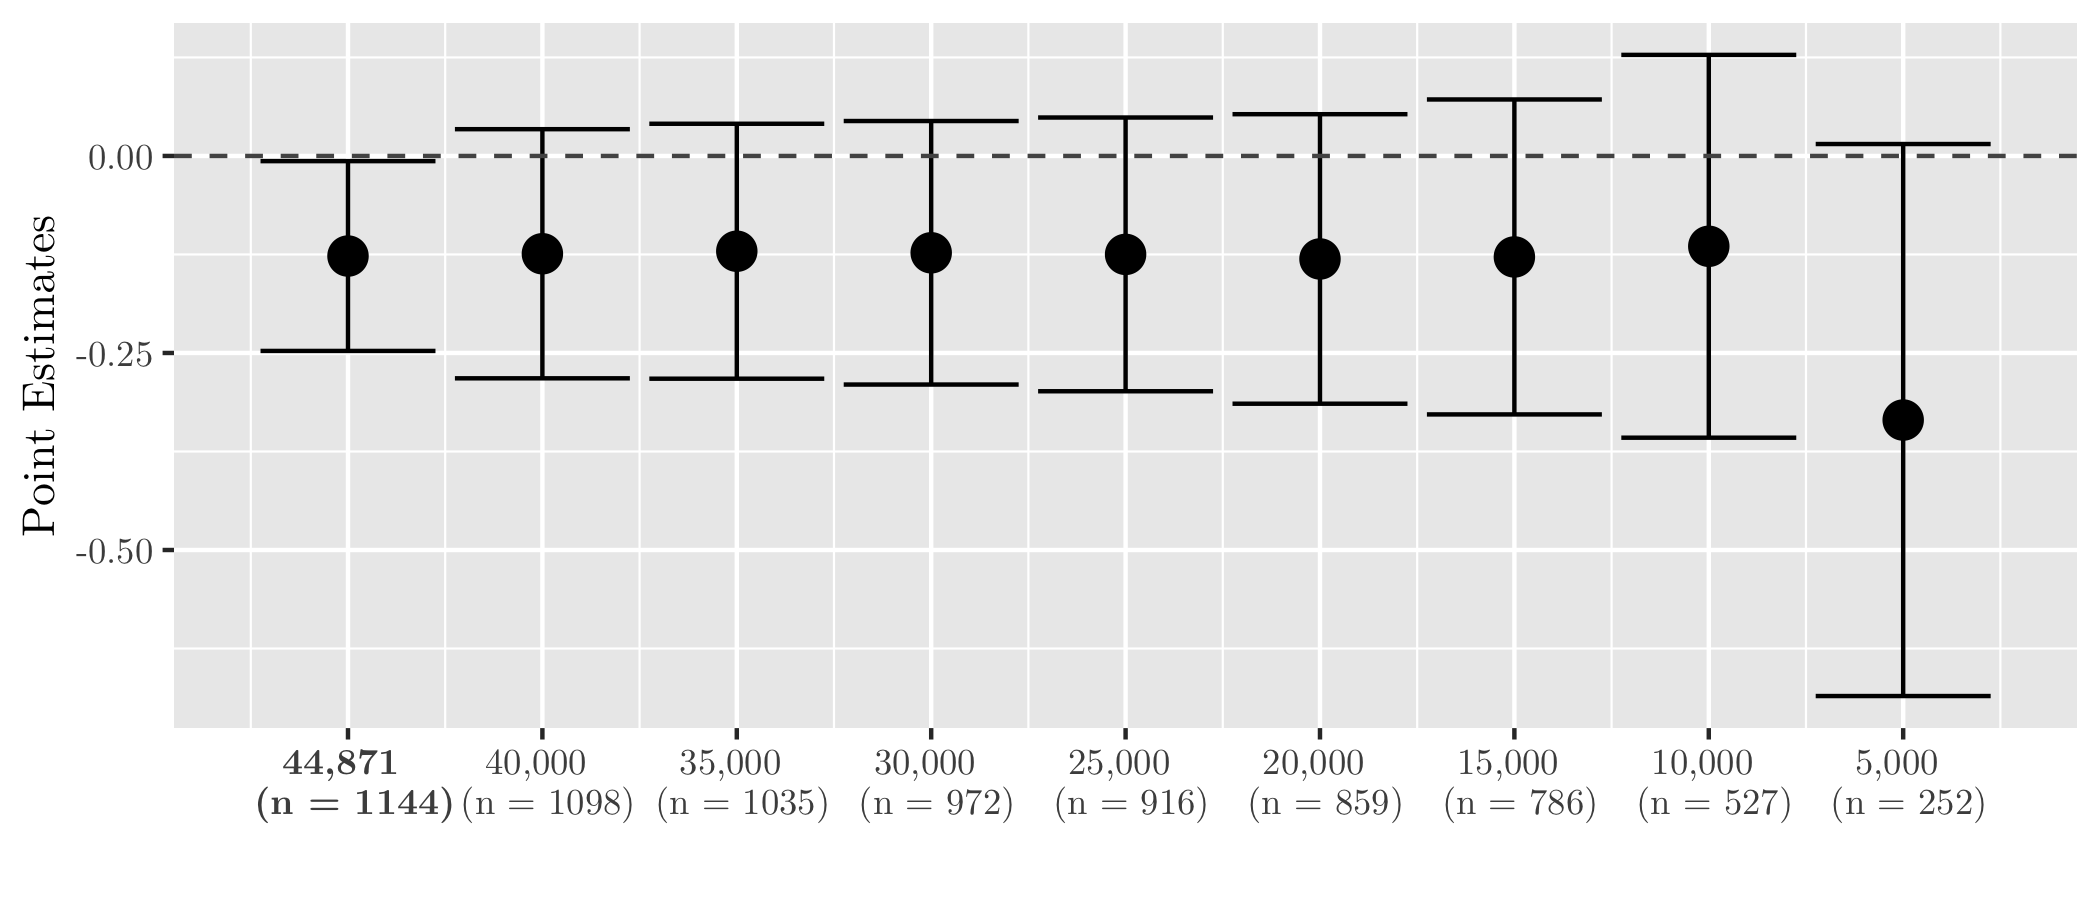
\includegraphics{./images/02falsificationplot1.png}
\caption{Mismanagement Binary Placebo 2}
\end{figure}

\end{frame}

\begin{frame}{Conclusion}
\protect\hypertarget{conclusion}{}

We test, but find no evidence, that discretion in public spending
reduces corruption.

A simple, back-of-the-envelope, calculation of the costs and benefits of
the procurement law in Brazil points to a small \textbf{5.98\%
prevention of resource misallocation}.

We speak to the literature of political decentralization, but instead of
looking at shared responsibility across government levels, we focus at
effect of sharing more (or less) responsibility with street-level
bureaucrats.

Not discussed in this presentation\ldots{} but we developed a method of
text analysis to read in each transfer and assign it to procurement
types (in appendix).

\end{frame}

\begin{frame}{Supplemental Material}
\protect\hypertarget{supplemental-material}{}

\end{frame}

\begin{frame}{Summary Statistics}
\protect\hypertarget{summary-statistics}{}

\begin{figure}
\centering
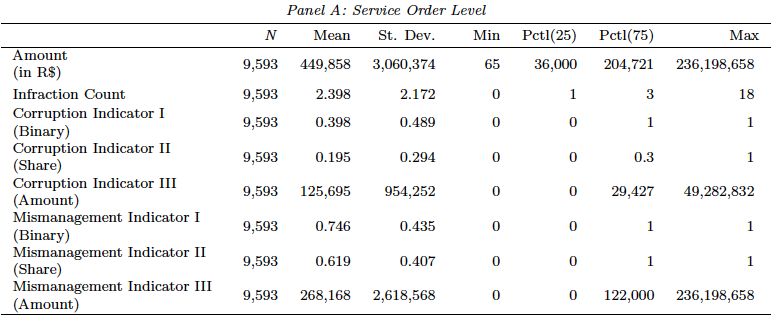
\includegraphics{./images/panelA.png}
\caption{Panel A: Variables at the Service Order Level}
\end{figure}

\end{frame}

\begin{frame}{Summary Statistics}
\protect\hypertarget{summary-statistics-1}{}

\begin{figure}
\centering
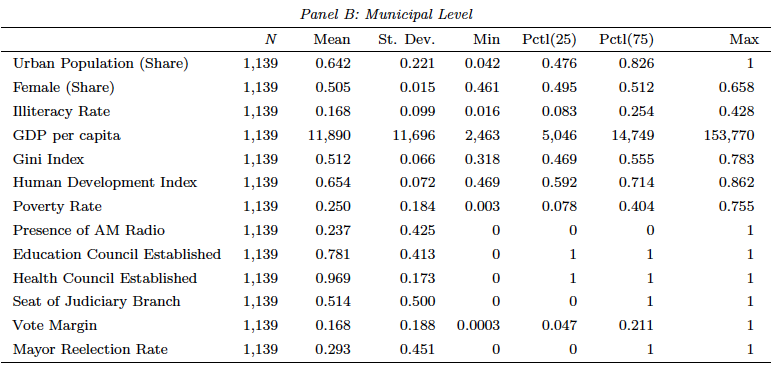
\includegraphics{./images/panelB.png}
\caption{Panel B: Variables at the Municipal Level}
\end{figure}

\end{frame}

\begin{frame}{Covariate Balance Tests}
\protect\hypertarget{covariate-balance-tests}{}

\begin{figure}
\centering
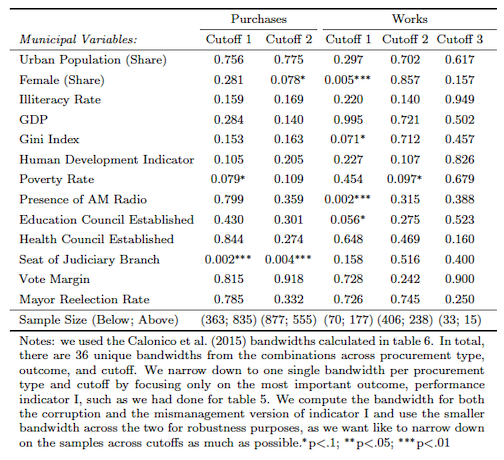
\includegraphics[width=0.75\textwidth,height=\textheight]{./images/covariates.png}
\caption{Covariate Balance}
\end{figure}

\end{frame}

\begin{frame}{Bandwidth Tests}
\protect\hypertarget{bandwidth-tests}{}

\begin{figure}
\centering
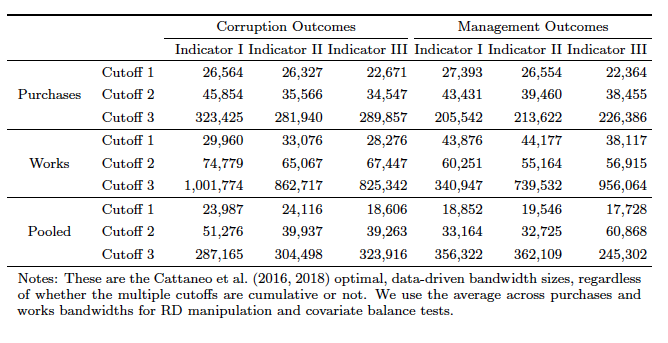
\includegraphics{./images/bandwidth.png}
\caption{Bandwidth Tests}
\end{figure}

\end{frame}

\begin{frame}{Mismanagement Share}
\protect\hypertarget{mismanagement-share}{}

\begin{figure}
\centering
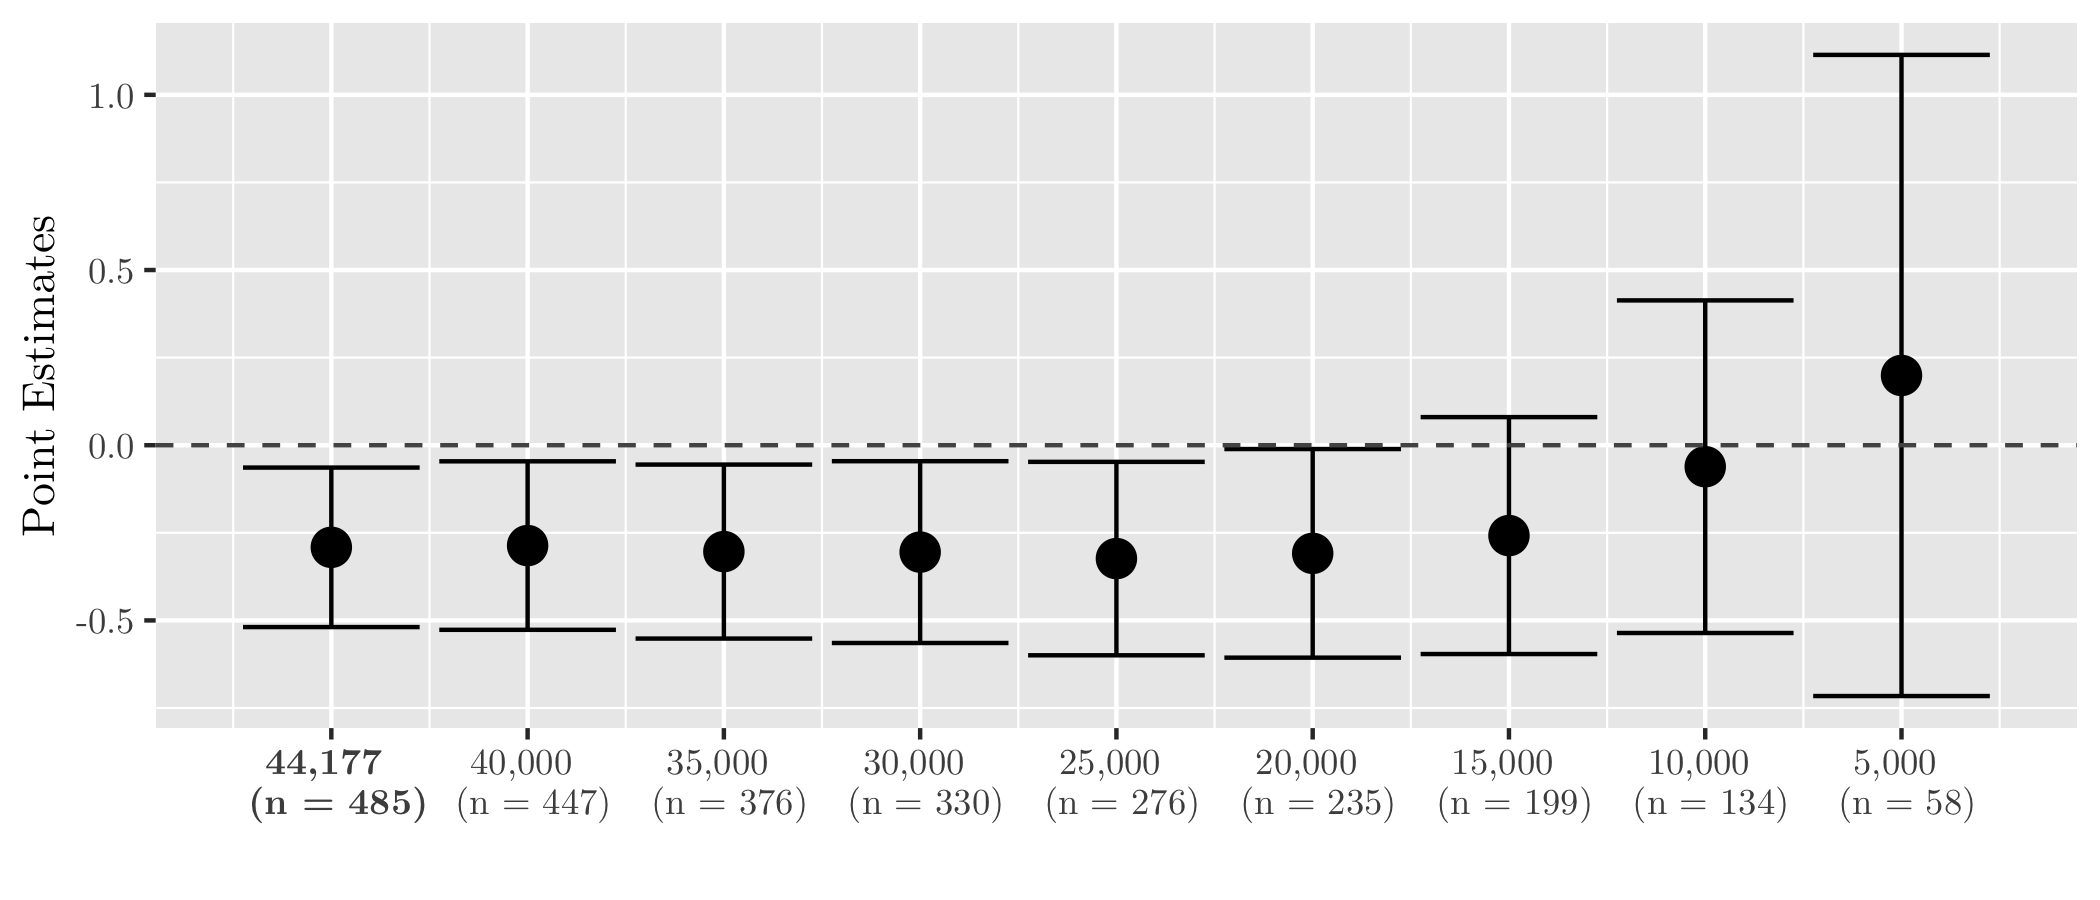
\includegraphics{./images/mismanagementplot2.png}
\caption{Outcome 2}
\end{figure}

\textbf{Interpretation:} reducing the discretion with which public
agents hire private contractors for public works projects reduces the
share of mismanagement problems found by auditors by \textbf{29.1
percentage points}.

\end{frame}

\begin{frame}{Mismanagement Amount}
\protect\hypertarget{mismanagement-amount}{}

\begin{figure}
\centering
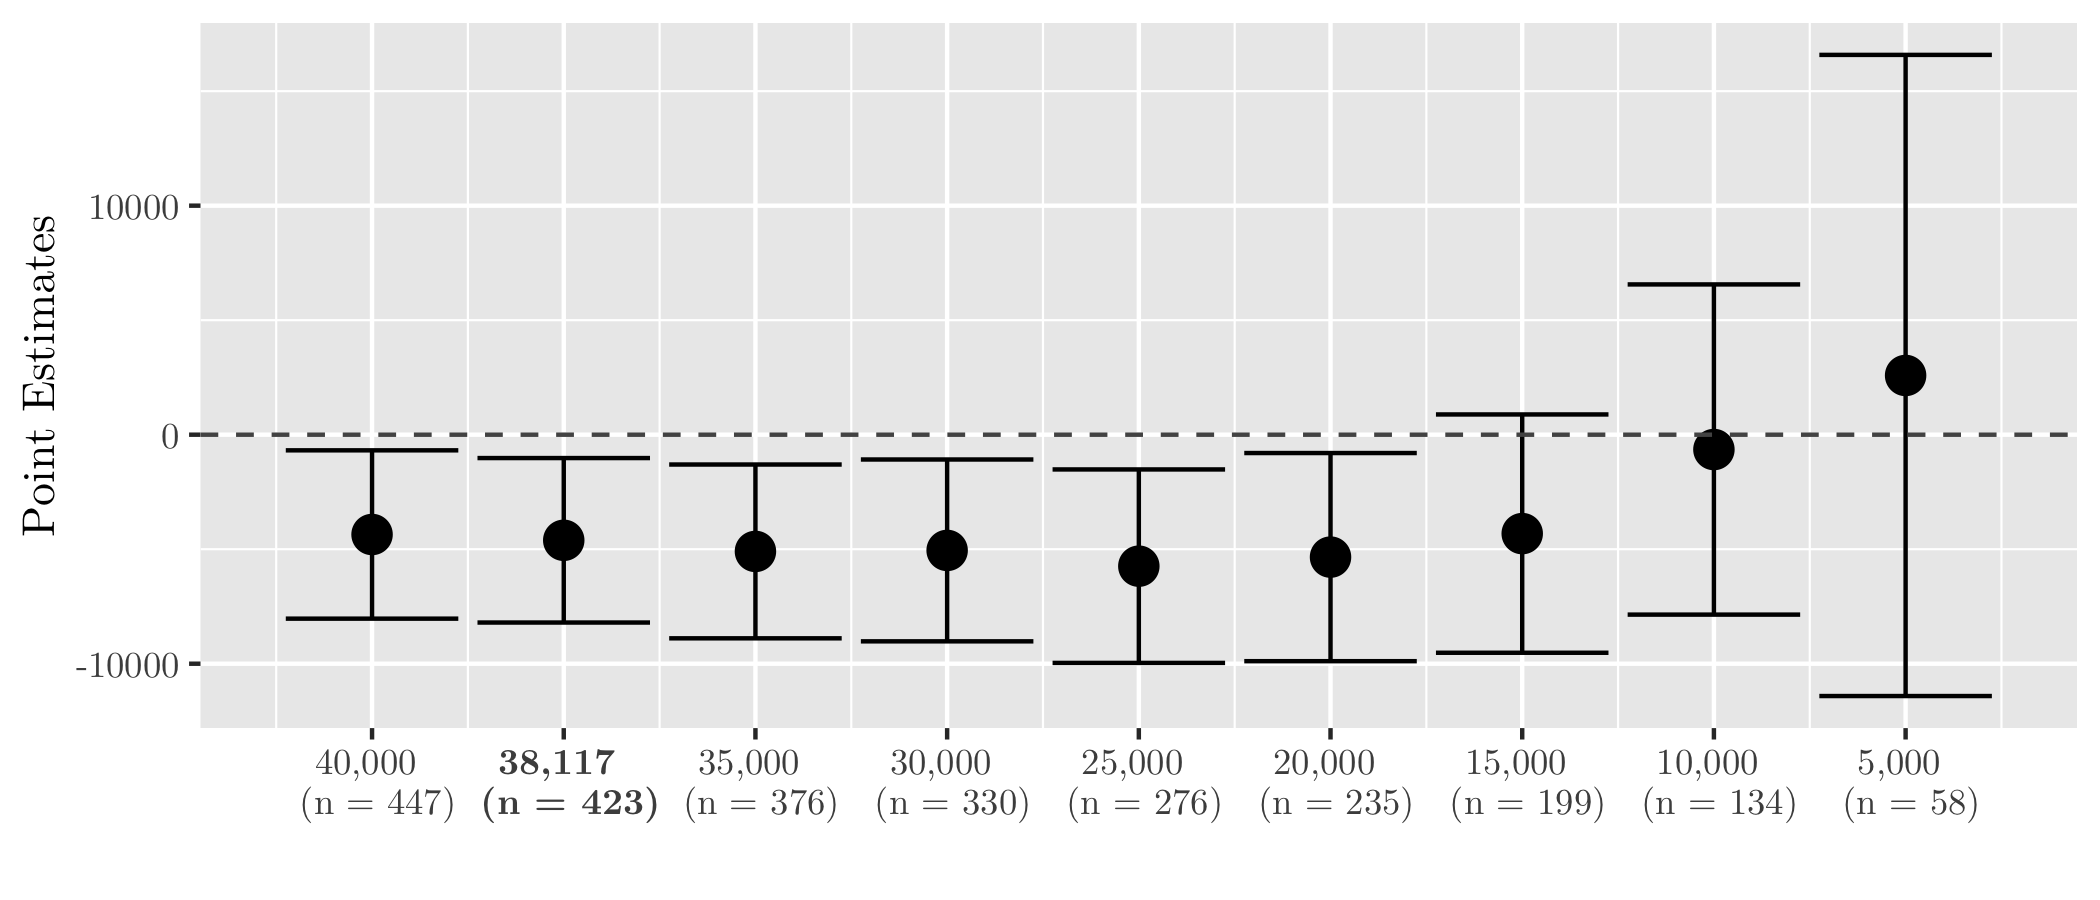
\includegraphics{./images/mismanagementplot3.png}
\caption{Outcome 3}
\end{figure}

\textbf{Interpretation:} reducing the discretion with which public
agents hire private contractors for public works projects reduces the
amount lost to mismanagement by \textbf{R\$4,611} (\textbf{\$1,155}
using the current exchange rate).

\end{frame}

\begin{frame}{Falsification Tests 1}
\protect\hypertarget{falsification-tests-1-1}{}

Is this result spurious? Using \textbf{fake purchases} cutoffs for works
transfers, the answer is \textbf{no}.

\textbf{Mismanagement Share}

\begin{figure}
\centering
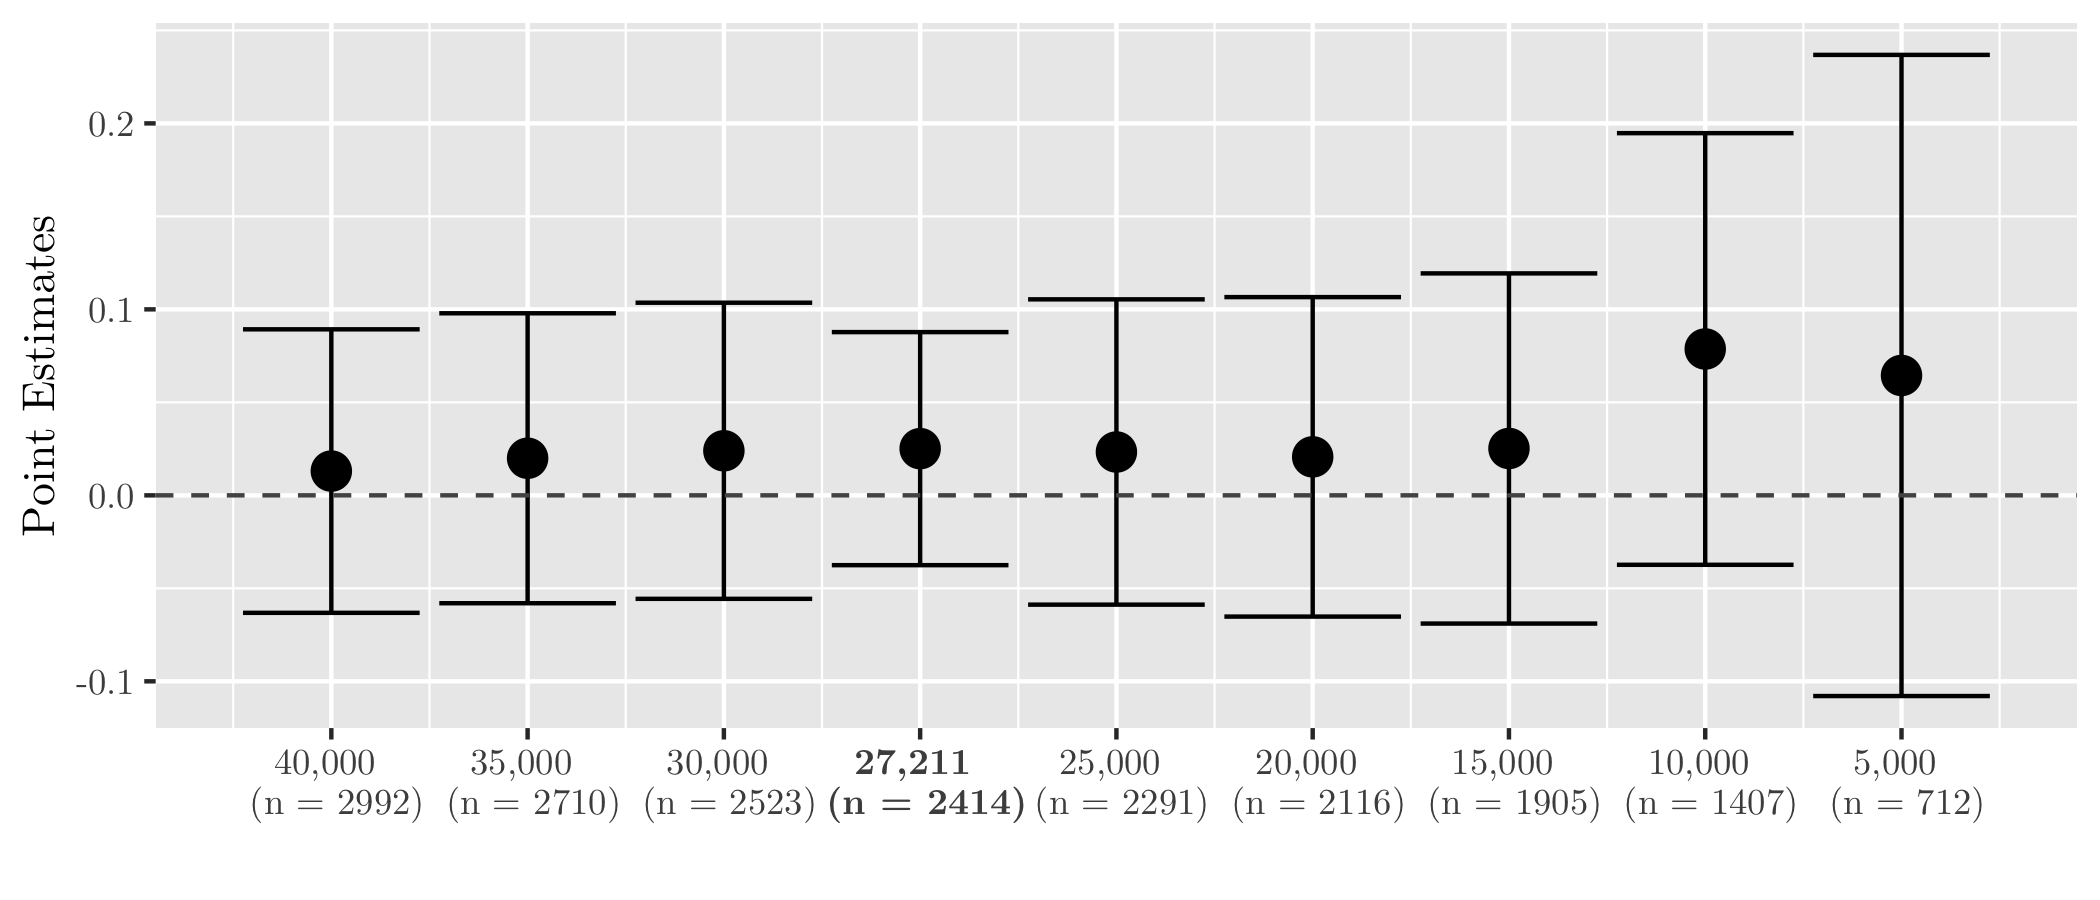
\includegraphics{./images/01falsificationplot2.png}
\caption{Placebo 2}
\end{figure}

\end{frame}

\begin{frame}{Falsification Tests 1}
\protect\hypertarget{falsification-tests-1-2}{}

Is this result spurious? Using \textbf{fake purchases} cutoffs for works
transfers, the answer is \textbf{no}.

\textbf{Mismanagement Amount}

\begin{figure}
\centering
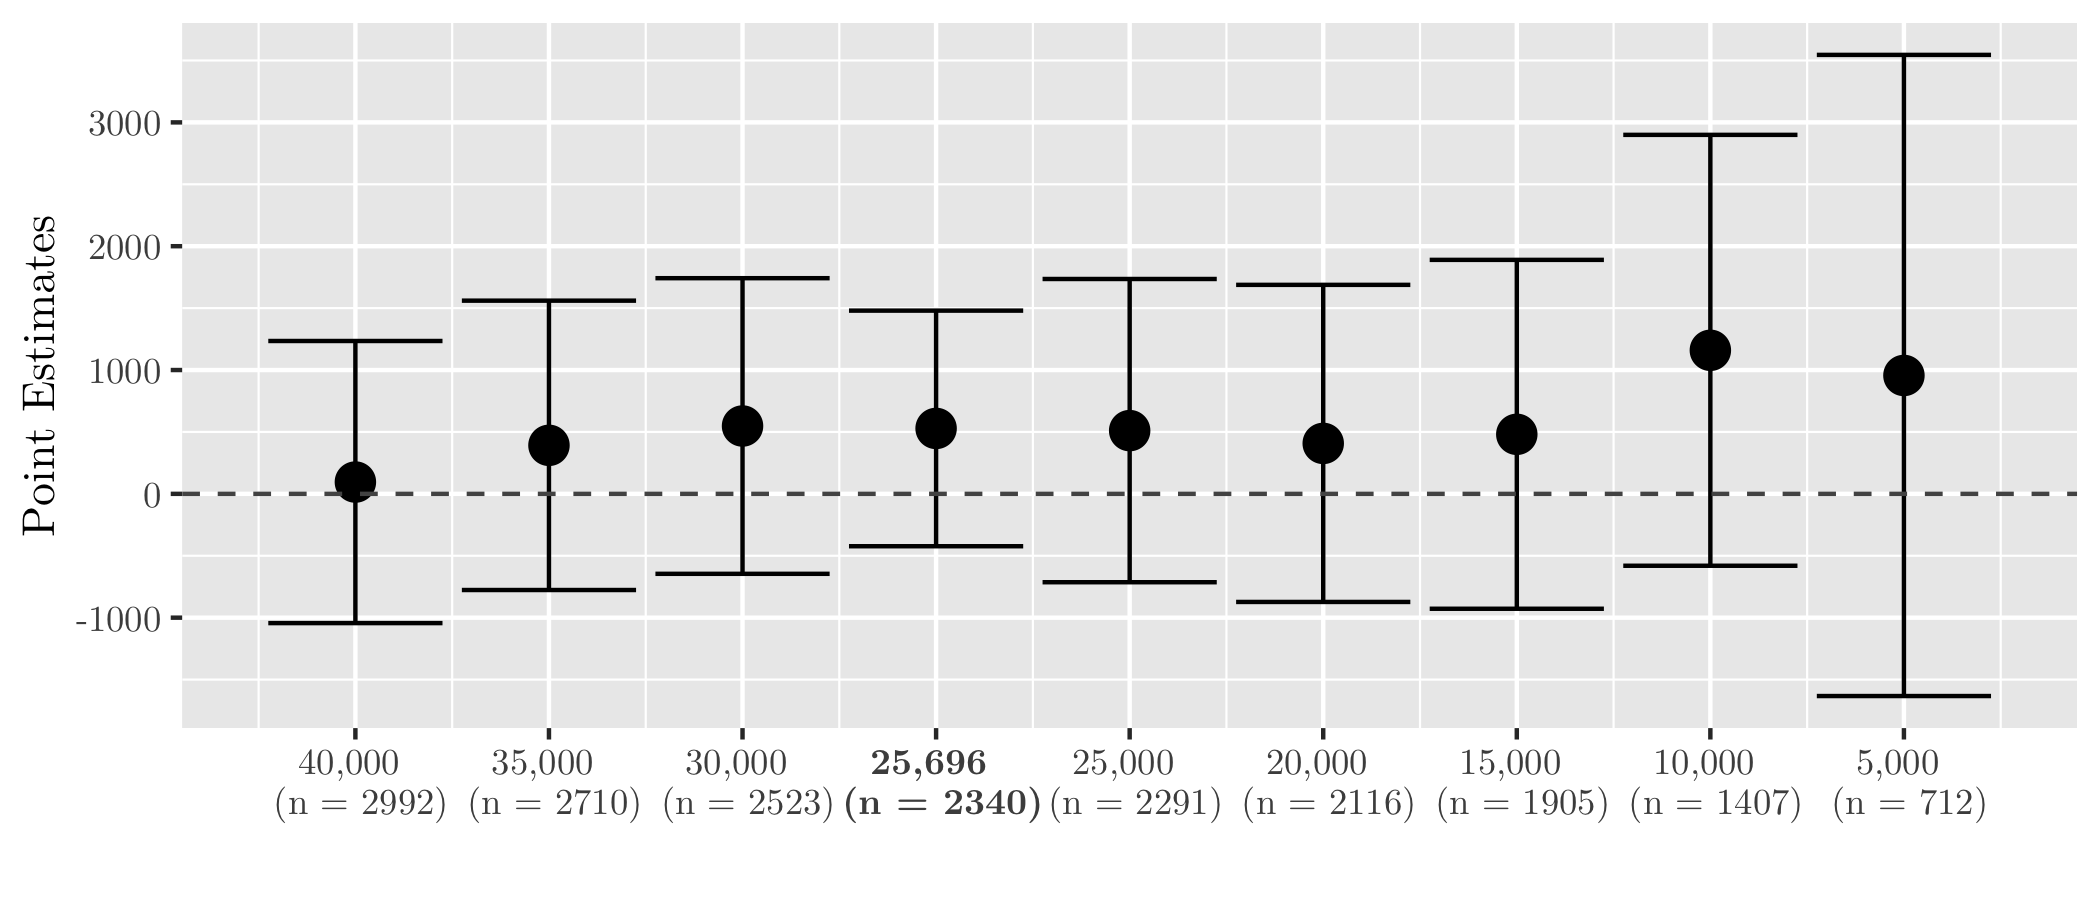
\includegraphics{./images/01falsificationplot3.png}
\caption{Placebo 3}
\end{figure}

\end{frame}

\begin{frame}{Falsification Tests 2}
\protect\hypertarget{falsification-tests-2-1}{}

Aren't we mixing up purchases and works transfers and picking up a
confounding effect? Using \textbf{non-procurement} transfers, the answer
is also \textbf{no}.

\textbf{Mismanagement Share}

\begin{figure}
\centering
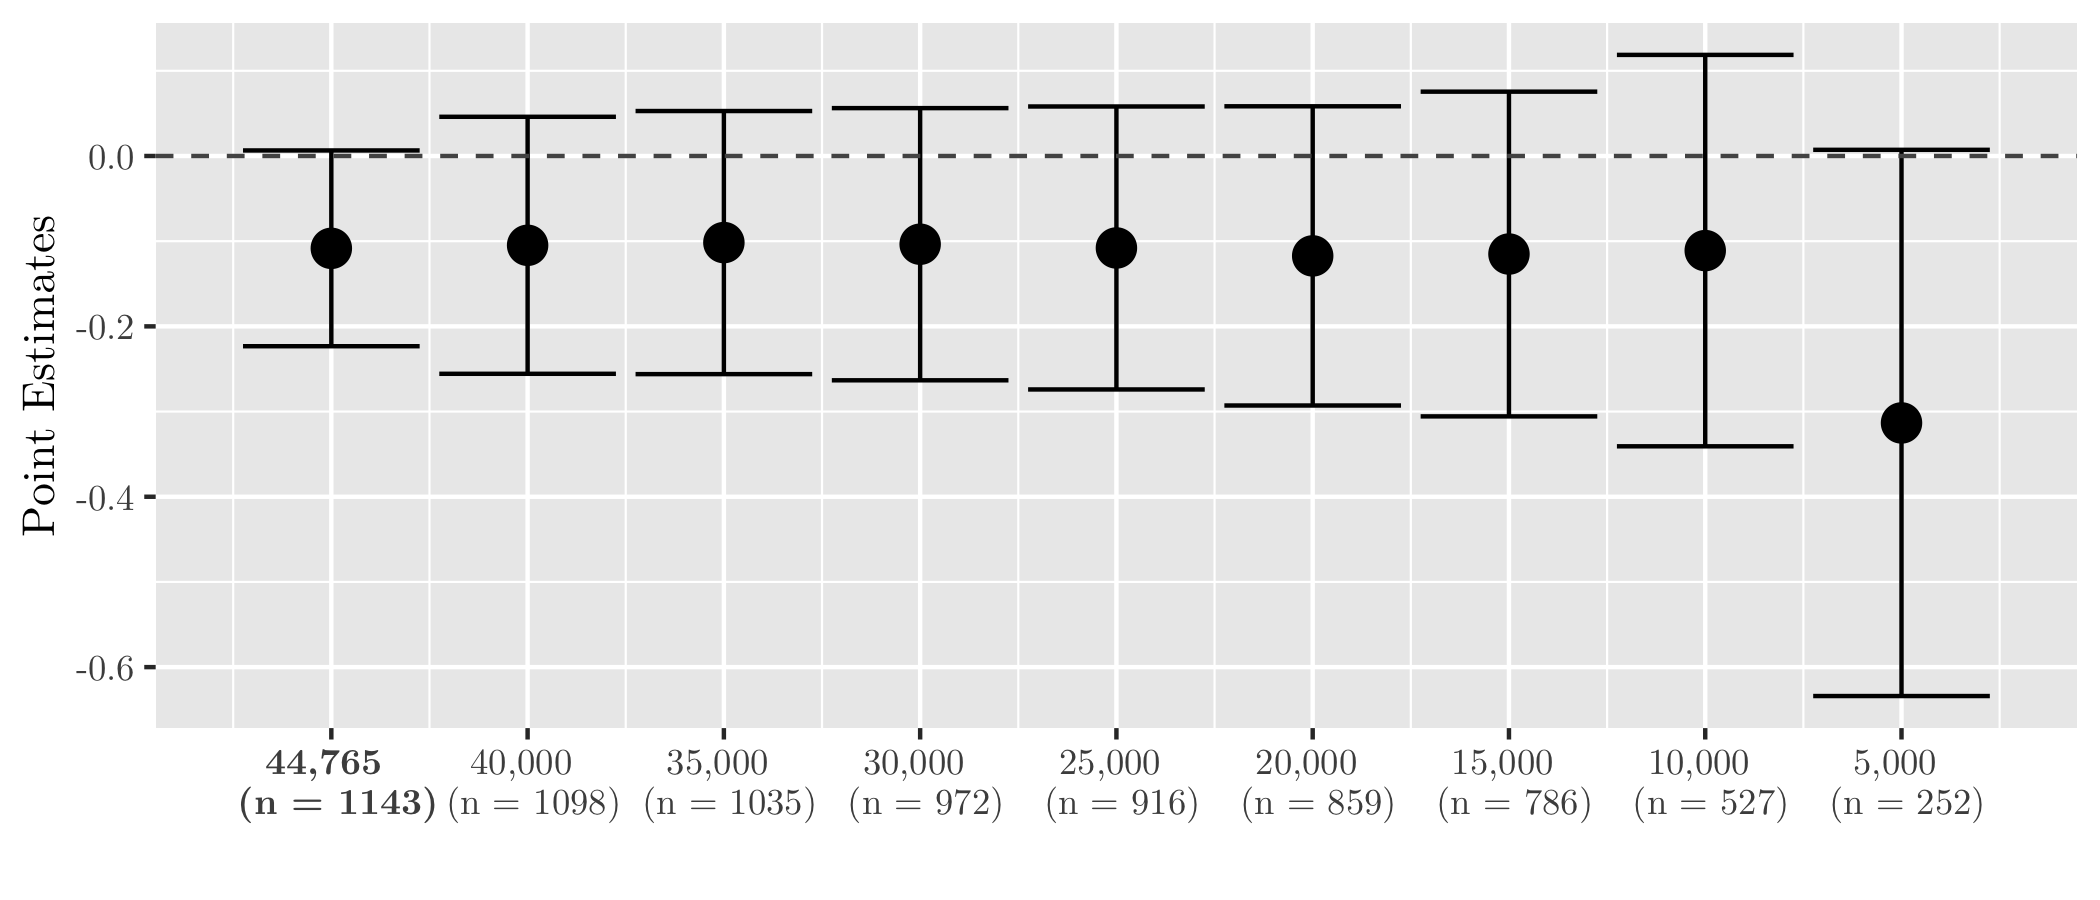
\includegraphics{./images/02falsificationplot2.png}
\caption{Placebo 2}
\end{figure}

\end{frame}

\begin{frame}{Falsification Tests 2}
\protect\hypertarget{falsification-tests-2-2}{}

Aren't we mixing up purchases and works transfers and picking up a
confounding effect? Using \textbf{non-procurement} transfers, the answer
is also \textbf{no}.

\textbf{Mismanagement Amount}

\begin{figure}
\centering
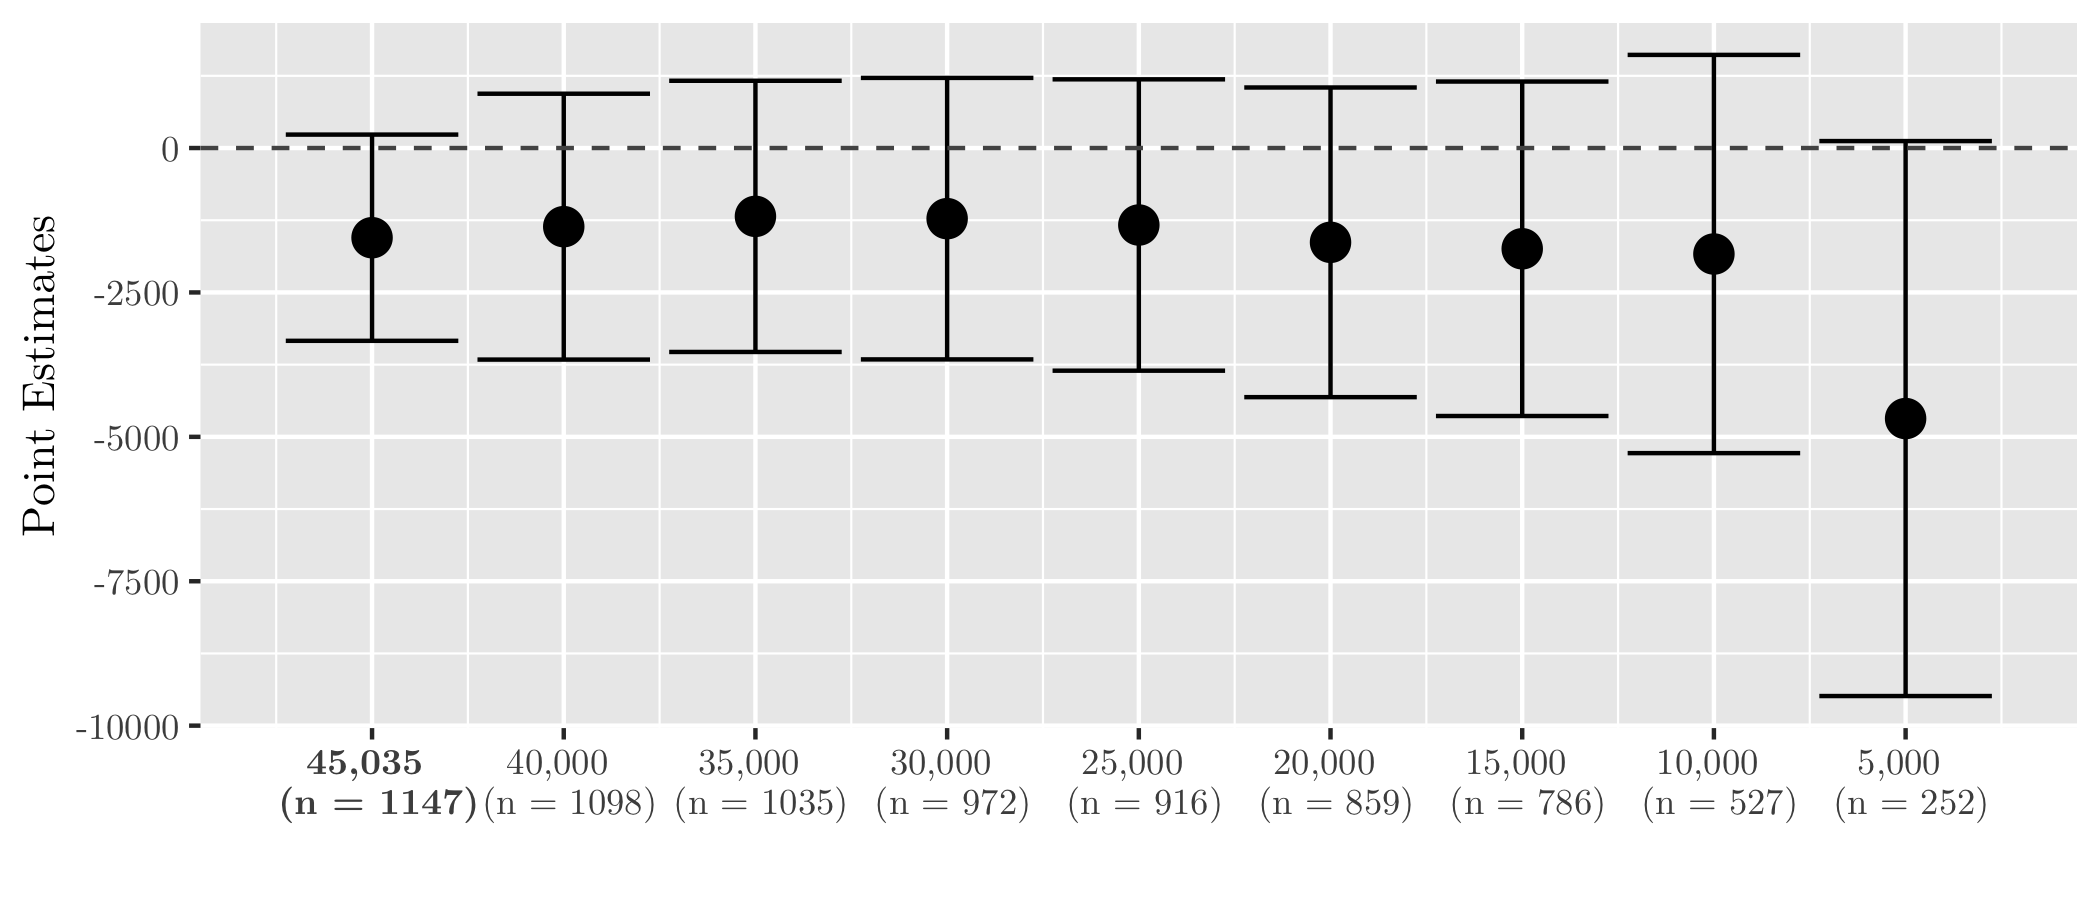
\includegraphics{./images/02falsificationplot3.png}
\caption{Placebo 3}
\end{figure}

\end{frame}

\begin{frame}{Cost-Benefit Analysis}
\protect\hypertarget{cost-benefit-analysis}{}

\begin{figure}
\centering
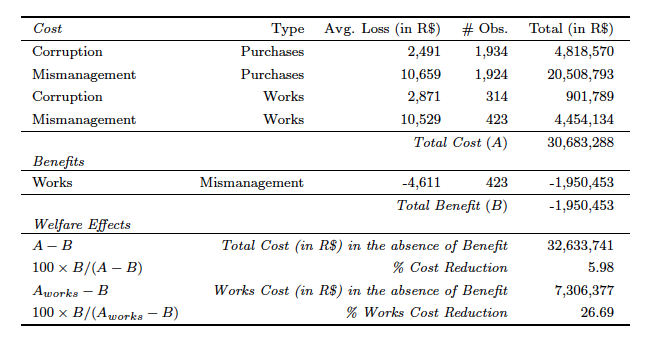
\includegraphics{./images/cba.png}
\caption{Back-of-the-envelope Calculation}
\end{figure}

\end{frame}

\begin{frame}{The End}
\protect\hypertarget{the-end}{}

\end{frame}

\end{document}
